\documentclass{article}
\usepackage{graphicx}
\usepackage{xcolor}
\usepackage{amsmath}
\usepackage{amsfonts}
\usepackage{amssymb}
\usepackage{tikz}
\usepackage{listings}
\usepackage{algpseudocode}

\usetikzlibrary{automata, arrows.meta, positioning}

\title{tut4}
\author{ntatsu}
\date{March 06, 2024}

\begin{document}

\maketitle

\section{Discussion}

\subsection{CFG}
Context-free grammars have rules, terminals, variables in comparison to a regular language.
\begin{itemize}
    \item $\text{Program} \, \rightarrow \epsilon \, \vert \, \text{Inst}; \, \text{Program}$
    \item $\text{Instruction} \, \rightarrow \, \vert \, \text{Assignment} \, \vert \, \text{if-else} \, \vert \, \text{While} $
    \item $\text{Assignment} \, \rightarrow \text{Variables}\, = \, \text{Arith Exp}$
    \item $\text{Variables} \, \rightarrow x \, \vert \, y \, \vert \, z \, \vert \, \dots$
    \item $\text{Arith Exp} \, \rightarrow \text{Variables} \, \vert \, \text{Number} \, \vert (\dots) \, \vert \, (\dots + \dots) \, \vert \, (\dots * \dots) \, \vert \, \dots$
\end{itemize}

\section{CFG}

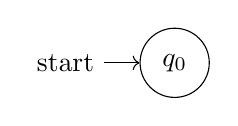
\begin{tikzpicture}
    \node [state, initial] {$q_0$};
\end{tikzpicture}

\end{document}

